\documentclass{beamer}
\usepackage[utf8]{inputenc}
\usepackage{utopia}
\usepackage[round]{natbib}
%\usepackage[
%backend=biber,
%style=plainnat,
%citestyle=authoryear
%]{biblatex}

\bibliographystyle{plainnat}

\usetheme{Madrid}
\usecolortheme{default}
\title[COMP5411 Rendering Project]{COMP5411 Rendering Project \\ Lens Renderer}
\author[Anshuman \& Aaron]{Anshuman Medhi \\ Aaron Si-yuan Wang}
\date{Group 21}

\begin{document}
\frame{\titlepage}

\begin{frame}
    \frametitle{Project Summary}
    \begin{block}{Rendering Lenses}
       \begin{itemize}
        \item Render a standard scene with objects and lighting, and include interactive magnifying lenses
        \item Simulate realistic refraction and dispersion of light to create all kinds of lens distortion
        \item Multipass rendering to handle multiple lens interaction
       \end{itemize} 
    \end{block}
\begin{figure}[htpb]
    \centering
        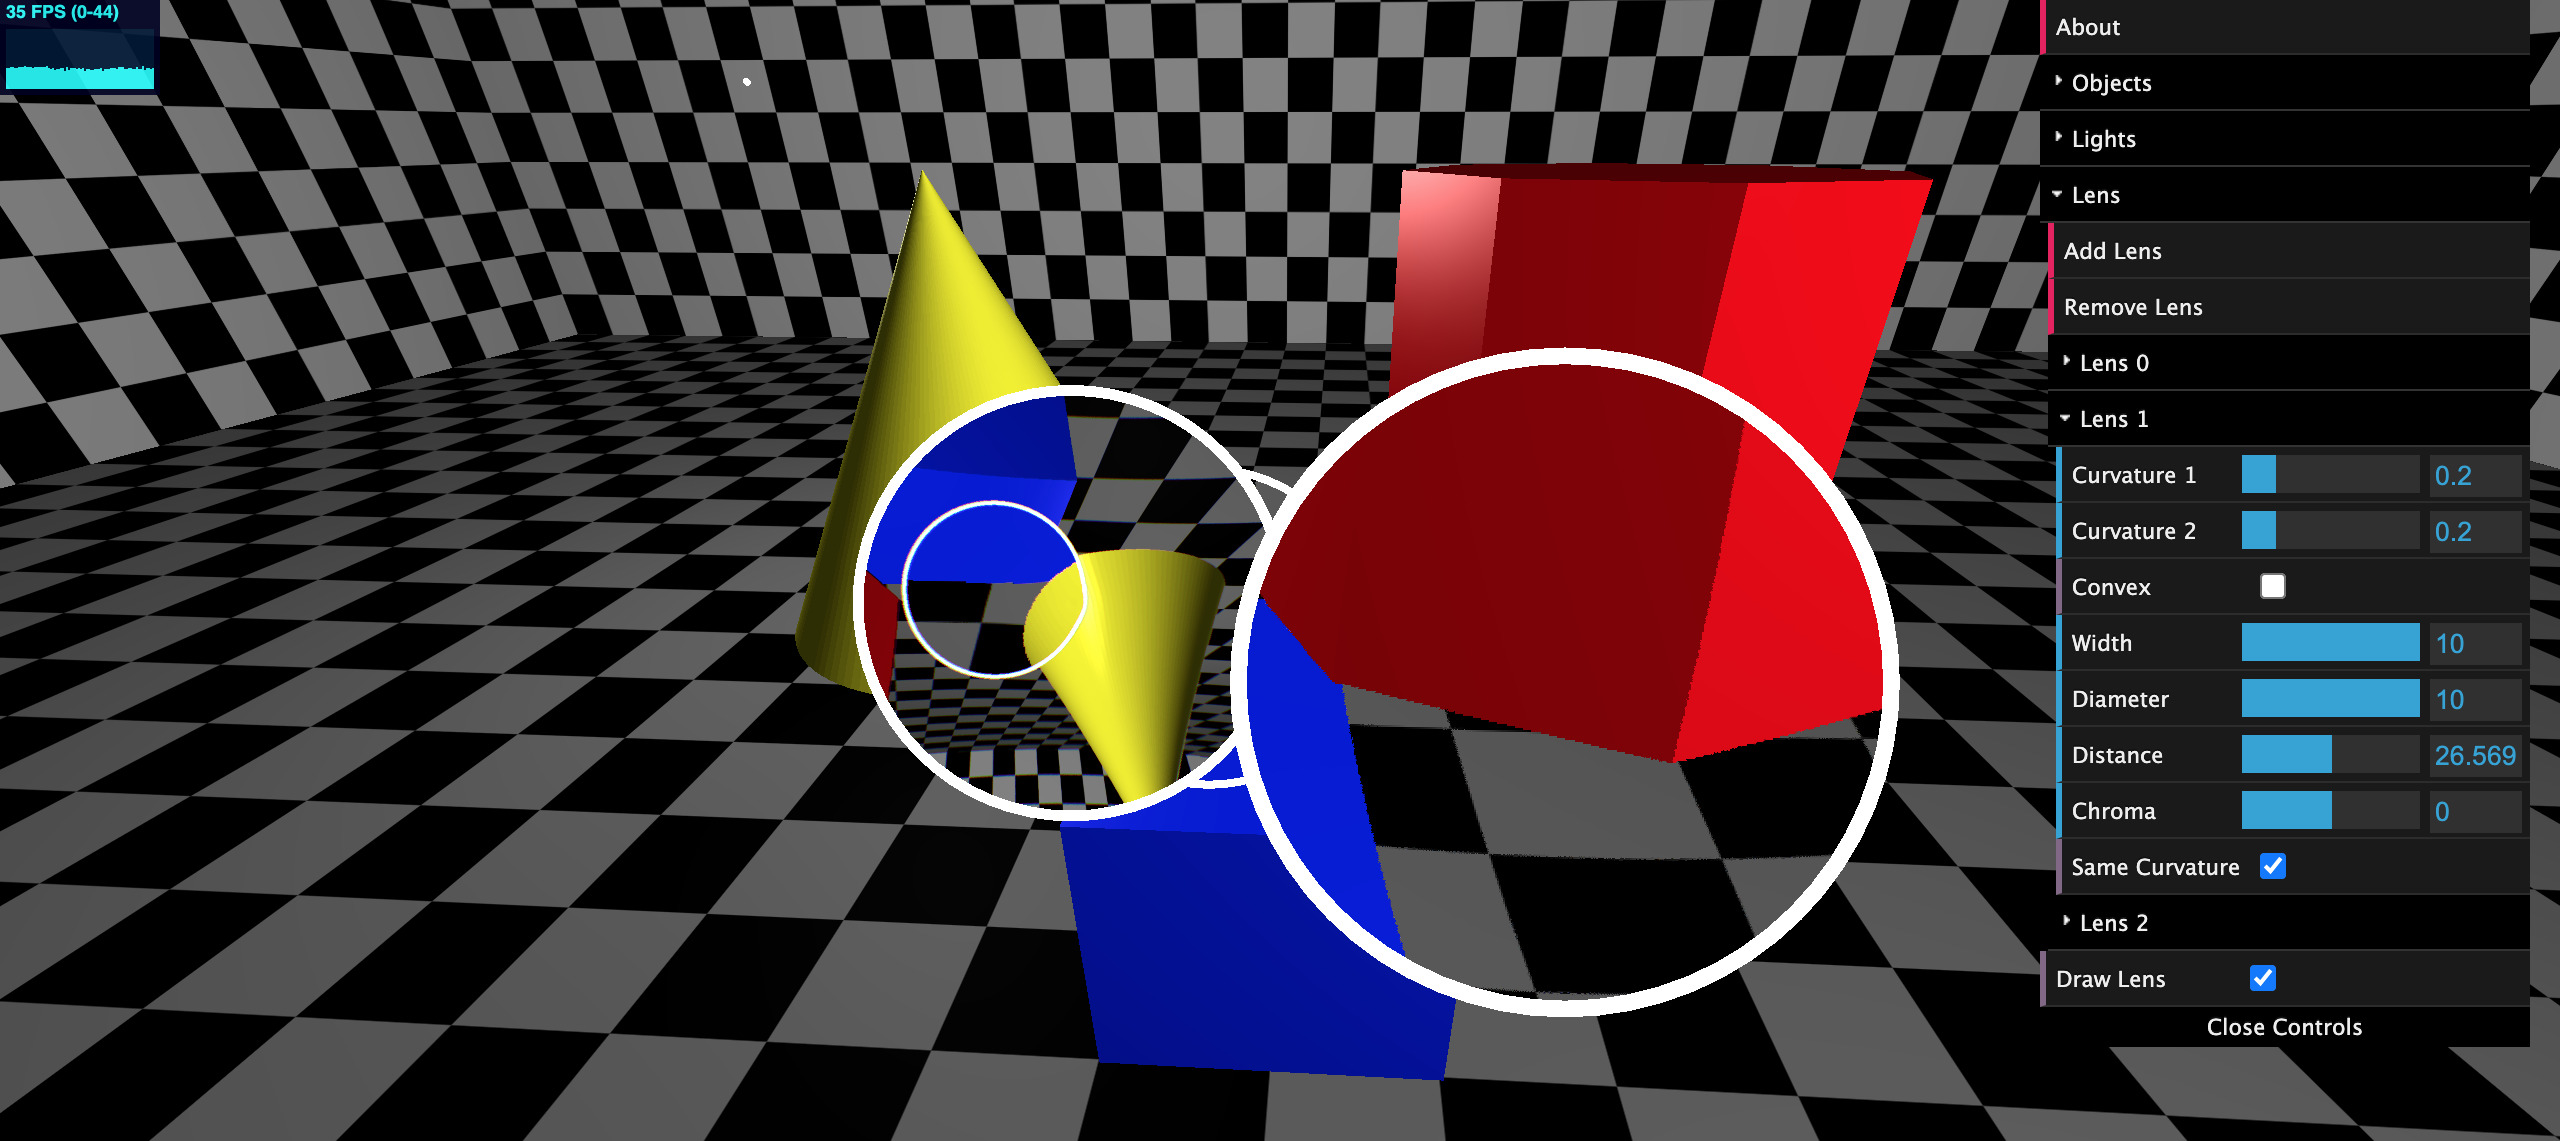
\includegraphics[width=0.7\textwidth]{images/main}
        %\label{fig:}
    \end{figure}
\end{frame}

\begin{frame}
    \frametitle{Project Summary}
    \begin{figure}[htpb]
        \centering
            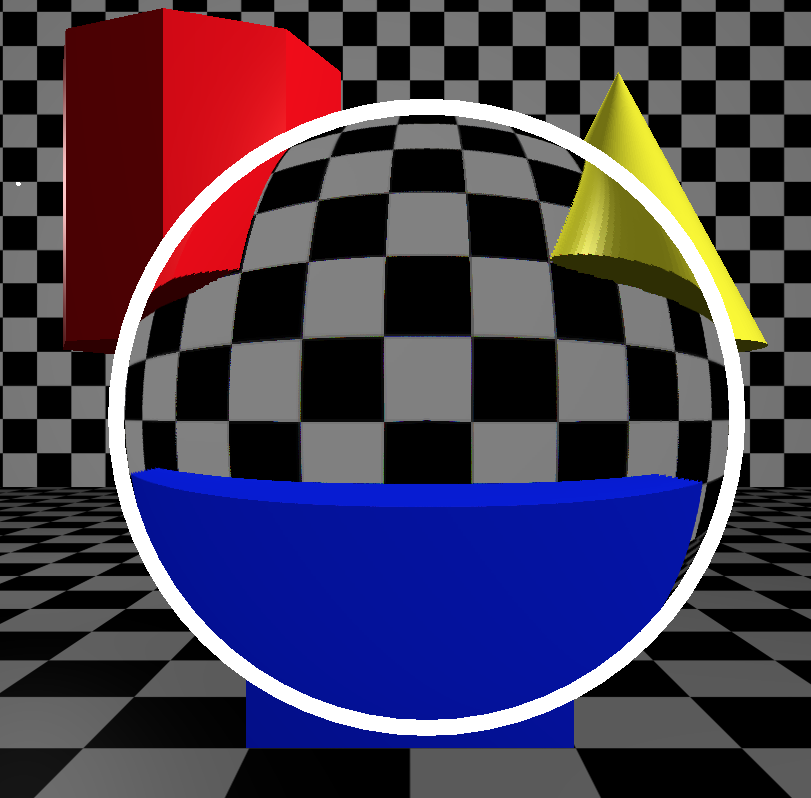
\includegraphics[height=0.35\textheight]{images/barrel}
            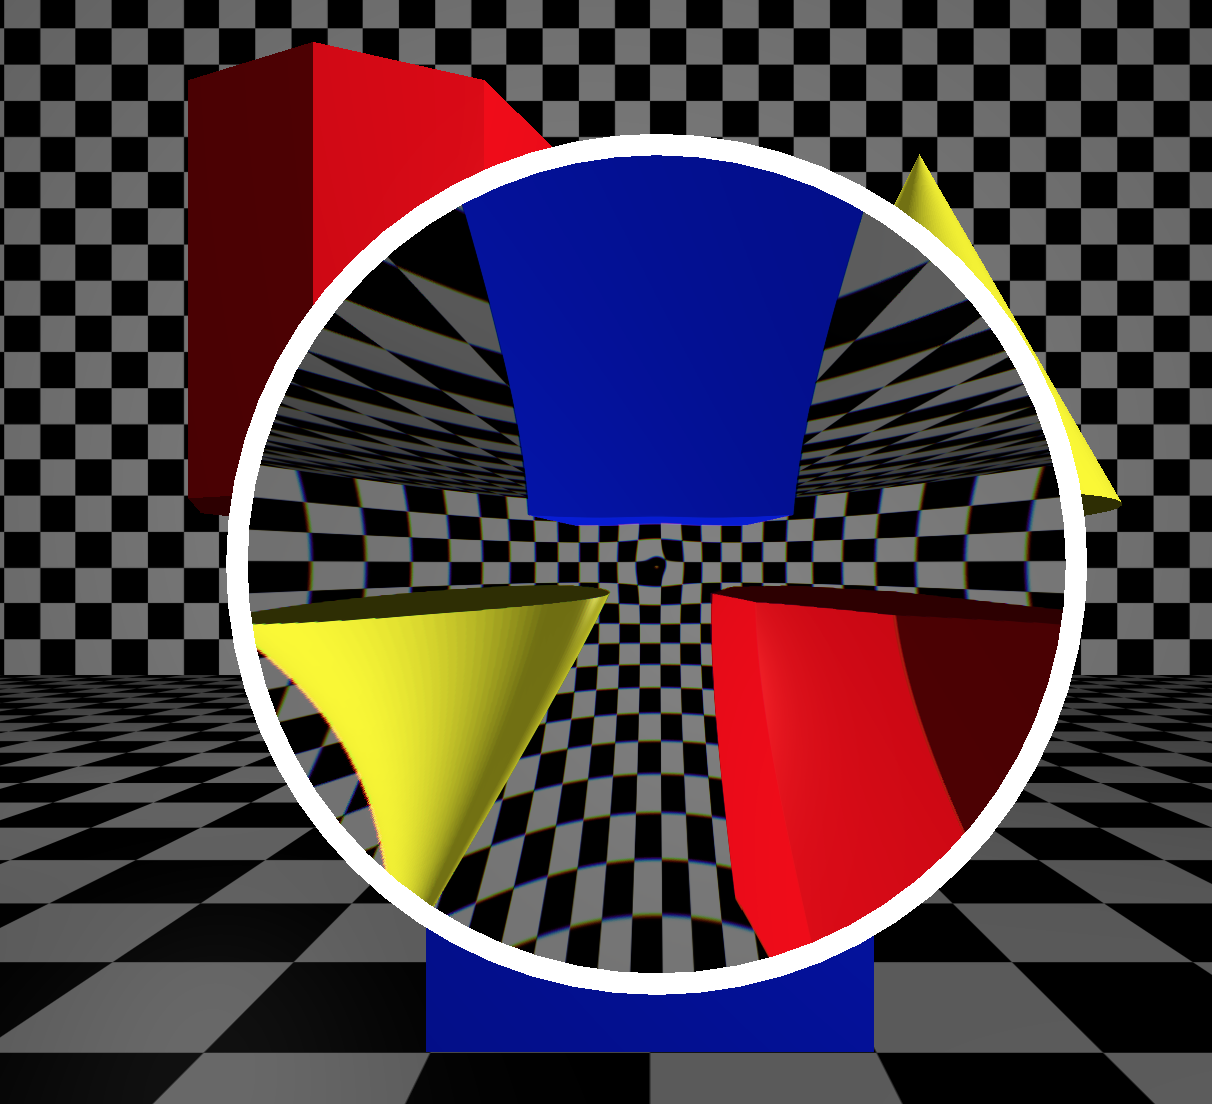
\includegraphics[height=0.35\textheight]{images/pincushion}\\
            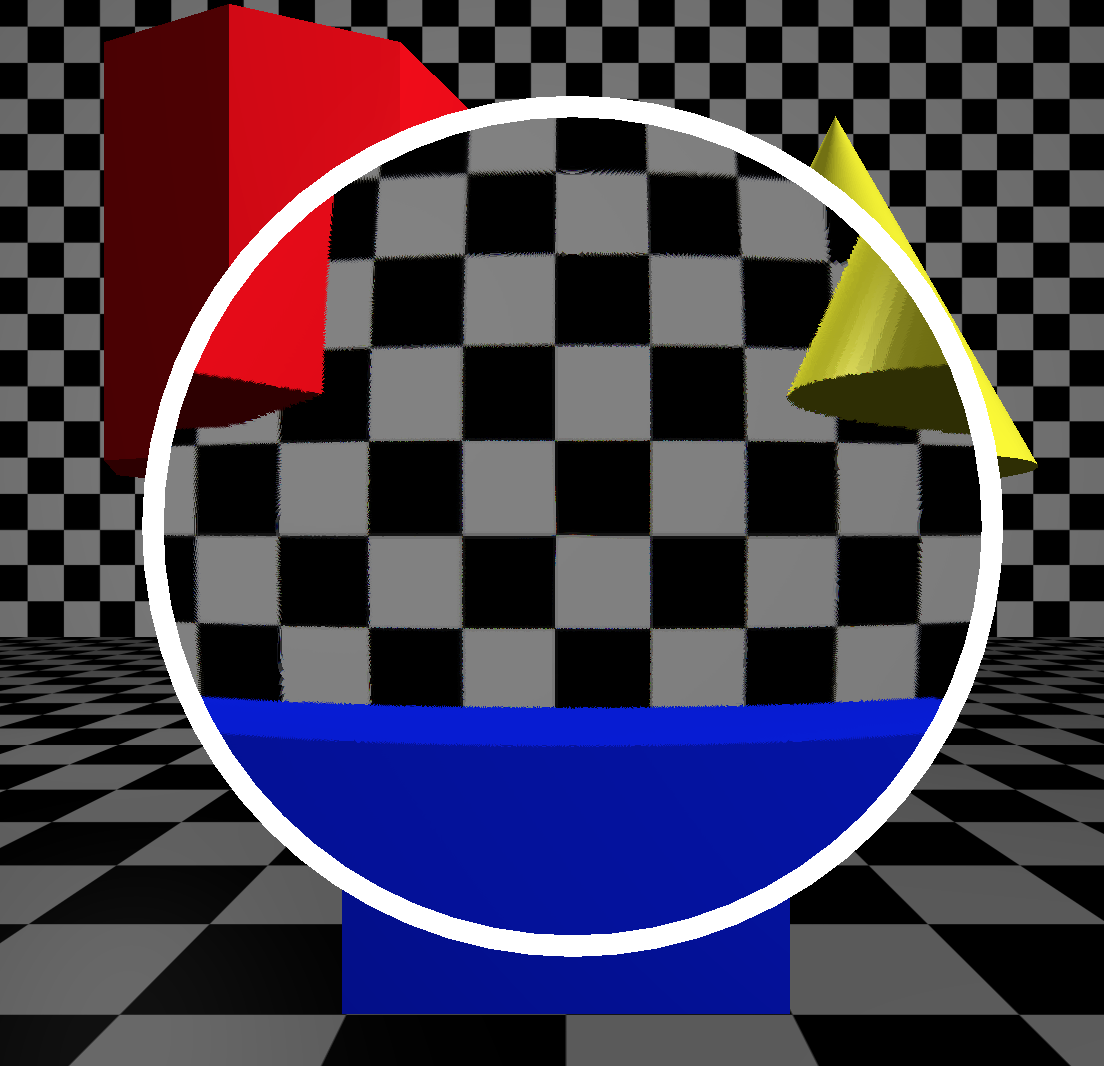
\includegraphics[height=0.35\textheight]{images/flat}
            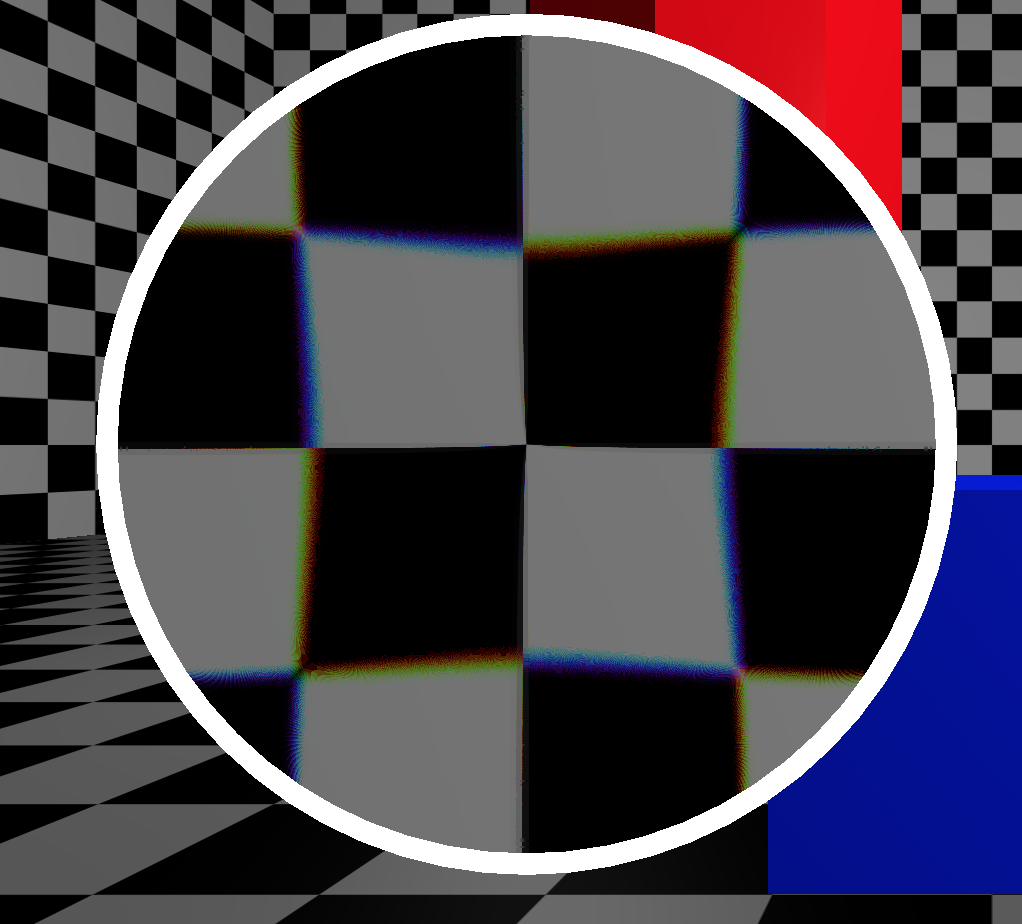
\includegraphics[height=0.35\textheight]{images/chroma}
        \caption{barrel, pincushion, and flat distortion, chromatic abberation}
        \end{figure}
\end{frame}
\begin{frame}
    \frametitle{Features}
    \begin{block}{Customizable Geometric Properties of Lens}
        \begin{itemize}
        \item Radius of curvature of each surface
        \item Diameter of lens
        \item Thickness of glass
        \item Position of lens
        \end{itemize}
    \end{block}
    \begin{block}{Customizable Scene Parameters}
        \begin{itemize}
            \item Phong shading parameters for each object
            \item Position of point lights
            \item Number of lenses
        \end{itemize}
    \end{block}
\end{frame} 

\begin{frame}
    \frametitle{Implementation}
    \begin{block}{Lens Fragment Shader}
        \begin{enumerate} 
            \item Find the center of each spherical cap of the lens
            \item Cast a ray through the lens onto the scene (a flat quad) refracting on the front and back surfaces
        \end{enumerate}
        \begin{figure}
            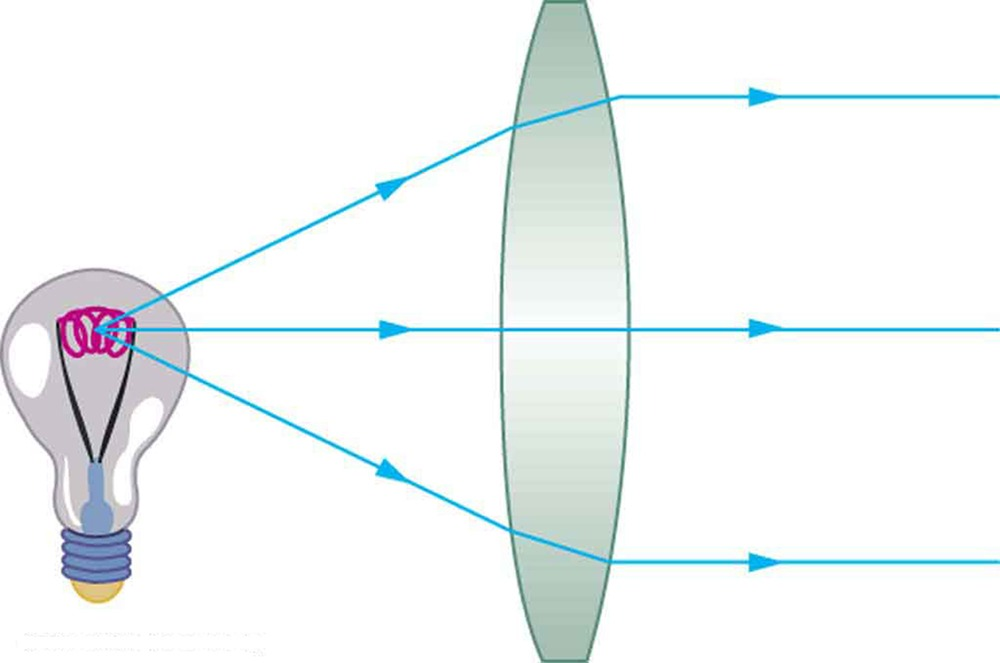
\includegraphics[height=0.4\textheight]{images/lens}
        \end{figure}
    \end{block}
\end{frame} 

\begin{frame}
    \frametitle{Implementation}
    \begin{block}{Lens Fragment Shader}
        \begin{enumerate} 
            \item Each color is refracted separately to handle dispersion effect 
        \end{enumerate}
            \begin{align*} 
                r &= \frac{R}{2} & g &= \frac{G}{2} & b &= \frac{B}{2}\\
                y &= \frac{2R+2G-B}{6} & c&=\frac{2G+2B-R}{6} & v&=\frac{2B+2R-G}{6}
            \end{align*}
            \begin{align*} 
                R &= r + \frac{2v+2y-c}{3} & G &= g + \frac{2y+2c-v}{3} & B &= b + \frac{2c+2v-y}{3}
            \end{align*}
    \end{block}
\end{frame} 
\begin{frame}[fragile]
    \frametitle{Implementation}
    \begin{block}{Multipass Rendering}
        \begin{enumerate}

        \item Render the original scene into a \verb|WebGLRenderTarget| texture $t_0$
        \item For each lens $i$ we create a new scene which consists of:
        \begin{itemize}
            \item Orthographically projecting the previous texture $t_{i-1}$ onto the next texture
            \item Using a \verb|CircleGeometry| with a custom shader material to distort a part of the previous texture $t_{i-1}$ 
            \item Blending the previous texture and the distorted circle together
        \end{itemize}
        \item Step 2 repeats for every lens, except the last lens does not render to a texture, but directly to a screen
        \item  We ensure that lenses are rendered in depth-order so that lenses can 'see' each other
        \end{enumerate}
    \end{block}
\end{frame} 

\end{document}
